\documentclass[twocolumn]{article}

\usepackage{csquotes}
\MakeOuterQuote{"}

\usepackage[backend=biber, bibstyle=ieee, url=false,
            giveninits=true, doi=false, maxbibnames=15]{biblatex}
\addbibresource{references.bib}

\usepackage{graphicx}
\usepackage{amsmath}
\usepackage{amssymb}
\usepackage{algorithm}
\usepackage{algorithmicx}
\usepackage[noend]{algpseudocode}
\usepackage{amsthm}
\usepackage[
    top=0.75in,
    bottom=0.75in,
    left=0.75in,
    right=0.75in
]{geometry}
\usepackage{mathtools}
\usepackage{float}
\usepackage{mathrsfs}
\usepackage{xspace}
\usepackage[f]{esvect}
\usepackage{bm}
\usepackage{xcolor}
\usepackage{hyperref}
\usepackage{enumitem}
\hypersetup{
    colorlinks=true,
    citecolor=.,
    linkcolor=.,
    urlcolor=.,
}


\title{\LARGE \textbf{Spatial Election Explorer (SEE)}}
\author{
    M. August Rossi,
    Michael Xiao,
    Emma Ross,
    Shu Luan \\
    {\small University of Chicago}
}

\begin{document}

\maketitle

\begin{figure*}
  \centering
  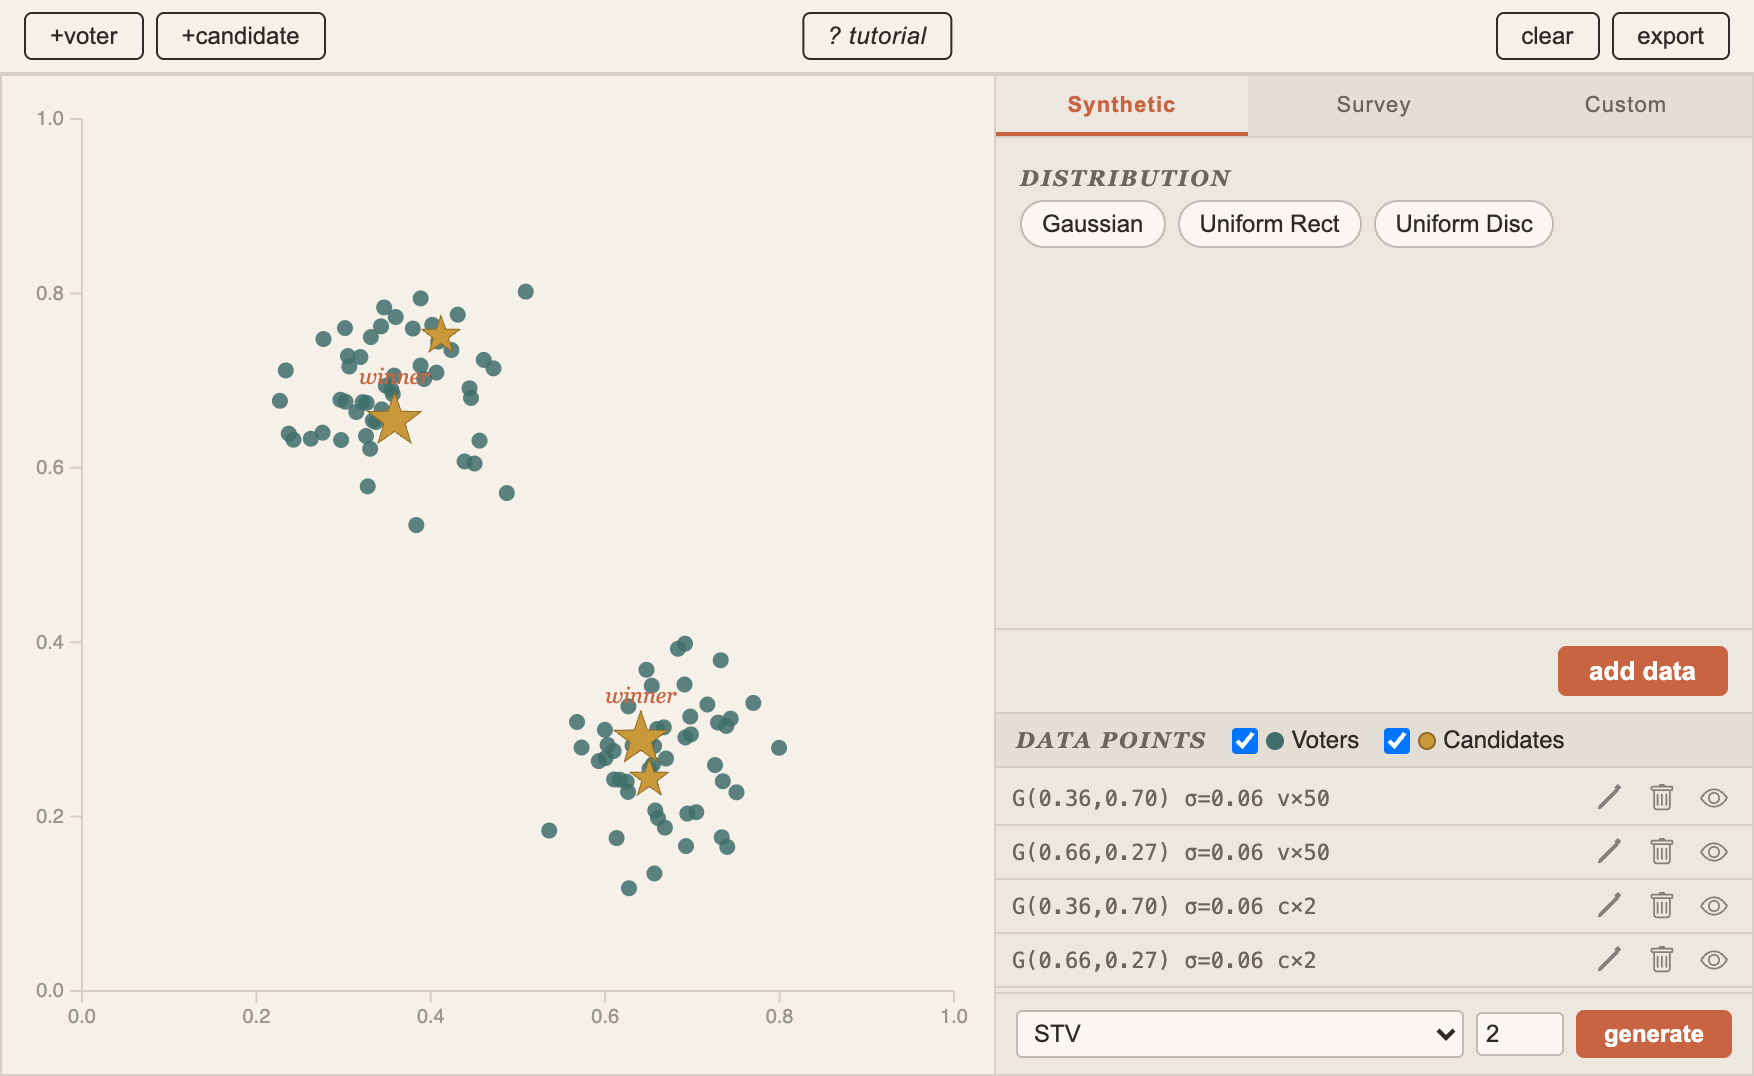
\includegraphics[width=0.7\textwidth]{img.png}
  \caption{Simulating a multi-winner STV election with the Spatial Election Simulator (SEE).}
  \label{fig:teaser}
\end{figure*}

\begin{centering}
  \textbf{Abstract.}
  We introduce Spatial Election Explorer (SEE),
an interactive web application for simulating ranked-choice elections on the Euclidean plane.
By encouraging users to iteratively build, experiment, and explore,
SEE helps them develop visual intuition about the properties and behavior of voting rules.

\end{centering}

\section{Introduction}%
\label{sec:Introduction}

Imagine a scenario in which some agents have each ranked a set of alternatives
from most preferred to least preferred.
How should this set of rankings be consolidated to a single ranking
or to a set of winning alternatives that fairly represents the entire group's preferences?
The most familiar setting for this problem is an election,
where voters rank candidates to choose their representatives,
but the problem setup applies much more broadly:
consider
a set of friends deciding what movie to watch or restaurant to visit;
a committee choosing what candidates to shortlist or hire; or
a panel of judges who have ranked competitors in ice skating or ballroom dance.

There are many algorithms (called \textit{voting rules}) for aggregating these group preferences:
how should the agents choose which to use?
Deliberation among the agents about this decision might rely on the details of the algorithms,
or on appeals to axiomatic properties that such algorithms may or may not satisfy.
They might say that STV is "more proportional" than Bloc Plurality for electing committees;
that IRV, unlike Plurality, "avoids the spoiler effect";
or that Plurality exhibits a "center squeeze" effect.
However, non-experts may find such arguments to be overly abstract.
Methods to visualize the behavior of voting rules can bridge this communication gap
and help voters develop intuition about the differences between algorithms.

The core objective of our project is to employ a previously developed technique
for visualizing elections as the basis of an interactive election simulator.
Allowing users to build, experiment, and iterate upon their own simulations
builds intuition in ways that a set of static plots cannot.
Combining visualization with iterative experimentation
allows users to both \textit{see} the properties of the various algorithms
and to learn the conditions under which these properties emerge.

\vspace{ 1em }
\textbf{Our Methodology.}
To facilitate visualization, we adopt a two-dimensional spatial model of voters' preferences.
Voters and candidates are jointly embedded in the Euclidean plane,
and voters rank candidates in order of increasing distance.
Voters therefore prefer candidates that are "similar" to themselves.
This model is common in both theoretical \cite{spatial}
and empirical \cite{guide} research in computational social science.
Further, it has a natural interpretation:
the position of voters and candidates might represent their
positions on two political issues or on two ideological axes.

% TODO: 1. overly wordy // 2. use active voice
In the Spatial Election Explorer (SEE),
voters and candidates can be placed on the plane by hand
or by sampling from the available distributions.
Their positions determine a unique collection of rankings,
which can be used as input to any of various voting rules.
The winners are displayed, providing the user a visual description
of how the distribution of winners differs according to the choice of voting rule.

\textbf{Audience.}
The intended audience for our application is threefold:
\begin{itemize}[nosep]  %[topsep=0.2em, itemsep=0.055555em]
\item[1.] Computational social choice (COMSOC) researchers can experiment with various voting rules,
testing and refining the intuition they already have for those methods.
Visualization may also suggest patterns of behavior in these voting rules that can
be axiomatized and studied formally.
\item[2.] Students studying social choice theory can use the tool to develop intuition
for the behavior of voting rules that supplements their learning in the
classroom. More aspirationally, perhaps they might be inspired to pursue
research in the area.
\item[3.] Policymakers and policy advocates who are considering the implementation of
ranked choice voting and wondering what voting rule to use might find value in
the tool as they develop intuition for the behavior of and tradeoffs between
the rules under consideration.
\end{itemize}

\textbf{Related Work.}
Our work is primarily inspired by Elkind et al. \cite{elkind},
whose experiments generated plots capturing the distribution of winning candidates
under various multi-winner voting rules
and across varying underlying distributions of voters and candidates.
%
Szufa et al. \cite{dap} created visual "maps" of preference profiles
by computing swap distances between ballots and applying the
multidimensional scaling (MDS) algorithm.


\section{Preliminaries}%
\label{sec:Preliminaries}
\input{prelim.tex}

\section{Application Design}%
\label{sec:Design and Implementation}

\subsection{Tutorial}%
\label{sub:Tutorial}
The tutorial serves to orient the user, introduce the voting rules,
and give the user a sense of how to interact with the application.

It begins by defining the spatial model, contextualizing the axes
as representing a policy or ideology space, and emphasizing the
key assumption: only the distance between voters and candidates matters
in determining how voters will fill out their ballots.

Next, it introduces the tool and the primary ways of using it
via a series of examples that introduce Plurality, Borda, IRV, and STV.
At each step, the tutorial shows an example plot
and asks the user to make a prediction of which candidate will win.

The plurality example demonstrates the well-known "spoiler effect",
in which a majority bloc of voters is shut out of representation
because they split their votes across multiple candidates,
while the minority bloc is unified in their support of a single candidate.

The Borda example explains how candidates are scored,
then demonstrates its tendency to elect centrist "consensus" candidates.

The IRV example shows how runoff voting can avoid the spoiler effect:
the plot is set up the same as in the plurality example,
but, in this case, one of the candidates supported by the majority bloc
wins the election.

Finally, the multi-winner example contrasts bloc plurality with STV.
It shows two clusters of voters, one slightly larger than the other,
with two candidates per voter cluster.
In bloc plurality, the larger cluster can sweep the election,
securing both seats on the committee, shutting out the other cluster entirely.
However, in STV, each cluster gets one seat on the committee---a more proportional outcome.

\subsection{Input}%
\label{sub:Input}
On the plot, voters are blue dots, and candidates are yellow stars.
There are four primary methods for placing voters and candidates on the plot.
\begin{itemize}
  \item \textbf{Manual Input.}
    The user can select to add a candidate or a voter,
    then click anywhere in the plot to add a point at that location.

  \item \textbf{Synthetic Sampling.}
    In the sidebar, the user can choose from any of the available distributions.
    They can set the distribution center by dragging it on the plot,
    or specifying the desired coordinate position in an input box.
    They can set distribution parameters with sliders or by entering
    the desired value in an input box.
    Then, they can set whether to sample voters or candidates,
    and set the number of points to be sampled.
    Finally, clicking "add data" adds these points to the plot.

    By stacking sets of samples drawn from different distributions,
    the user can easily create multiple clusters of voters or candidates.

    As in \cite{elkind}, the supported distributions are
    the Gaussian, the Uniform Rectangle, and the Uniform Disc.

  \item \textbf{Survey Data.}
    Upon selecting the "Survey" tab in the sidebar,
    the user can select two "Ideology" axes or political issues
    to serve as the axes of the plot.
    Then, they can sample voters from polling data.

    \item \textbf{Data Upload.}
    If a user has exported a JSON file of the points from a previously-generated plot,
    they may upload that data.
\end{itemize}

\subsection{Plot Management}%
\label{sub:Plot Management}
Every point manually added and every distribution sampled from
appears as a separate line item in the "Data Points" section of the sidebar.
The line describes the parameters that created it.
For every distribution line, the following interactions are available:
\begin{itemize}
  \item \textbf{Edit.}
    Highlights the distribution and reveals its settings;
    any of the settings (include type, count, position, and parameters)
    can be changed, and when the user clicks "update",
    the points are resampled.
    The user can click "cancel" at any point in this interaction
    if they want to keep the old settings.
  \item \textbf{Delete.}
    Removes this distribution.
  \item \textbf{Hide.}
    Hides this distribution; it is temporarily disabled
    for any election runs, but stays listed in the sidebar
    to be easily re-enabled later.
\end{itemize}
For any line item representing a manually-placed candidate or voter,
only the Delete and Hide options are available.

\subsection{Running Elections}%
\label{sub:Running Elections}
At the bottom of the sidebar, the user can choose their desired voting method,
select the number of winners, and run the election.
Running the election updates the plot,
making the winning candidates visually distinct from the others.


\subsection{Survey Data}%
\label{sub:Survey Data}

\subsection{Implementation}%
\label{sub:Implementation}
The application front end is built with Svelte and D3 in JS,
with Vite as the server.
The election algorithms are implemented in Python and
compiled to Web Assembly via Pyodide so that they can be run in browser.



\section{Future Directions}%
\label{sec:Future Directions}
\input{future-dir.tex}

\newpage
\printbibliography

\end{document}
